\section{eBPF Setup}\label{sec:ebpf_setup}
\subsection{Different BPF Programs}
\begin{figure}[htbp]
    \centering
    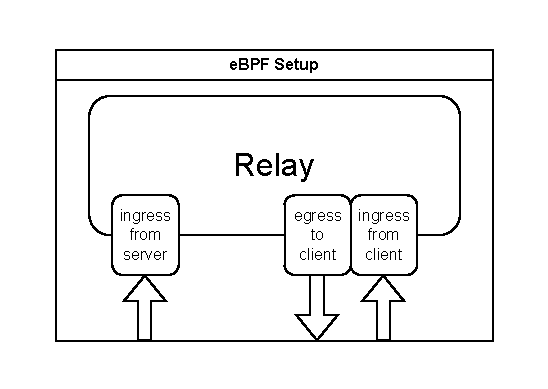
\includegraphics[width=7cm]{figures/03_fast_relays/ebpf-setup.drawio.pdf}
    \caption[Types of eBPF programs at relay]{The relay has to be equipped with three BPF programs.}\label{fig:ebpf-programs}
\end{figure}

In order to allow the relay to forward packets independently of the userspace, we
need to equip the relay with three BPF programs as seem in figure.
Those three programs are 
\begin{itemize}
    \item a program that handles incoming traffic \textbf{from} the clients (client ingress),
    \item a program that handles outgoing traffic \textbf{to} the clients (client egress) and
    \item a program that handles incoming traffic \textbf{from} the video server (server ingress).
\end{itemize}
Their responsibilities then are
\begin{itemize}
    \item handling the initial registration of new clients and storing their information such as
    MAC addresses in a BPF map,
    \item intercepting the packets from the video server, duplicating and redirecting them to 
    the egress program (as well as sending one unaltered packet to userspace for state
    management purposes),
    \item receiving the redirected packets at egress, altering them using the client specific
    data, deciding (based on packet priority and client congestion) if a packets should be dropped 
    or sent, storing info on sent out packets for future congestion control purposes and finally sending 
    them out to the clients.
\end{itemize}
This setup allows us to separate any state management and congestion control from the actual
packet forwarding and thus makes leaving out any immediate userspace processing possible.

Following is a more detailed description of the responsibilities of each of the three programs.
\subsubsection{Client Ingress} 
TODO
\subsubsection{Server Ingress}
TODO
\subsubsection{Client Egress}
The client egress program sees every packet that leaves the relay. 
This includes packets that have been redirected by the ingress program as well as packets that
have been generated by the relay itself.
Since the QUIC protocol works with packet numbers for a given connection it is necessary for 
the egress program to make sure the forwarded packets together with the userspace packets
provide a consistent state. 
For this the egress program maintains its own packet number counter for each connection.
That way only one counter has to be maintained and race conditions can be avoided.
However, this also means that the packets sent by the userspace are likely to have a different 
packet number than the one chosen by the QUIC library.
This might lead to inconsistencies again but can be avoided by not storing a packet from userspace
right away in the packet history but only once the BPF has stored it, along with the changed
packet number, in the map used for packet registration. % TODO: check if this is true / implemented
This initially gives a brief window where a packet was sent out but is not saved in the history
of the QUIC library but once the packet is then processed by the userspace routine handling the 
registration, any incoming ACKs for this packet can be processed correctly.
% TODO: retransmission? maybe use relay cache for that?
TODO

\subsection{Packet Registration}
In order to make the congestion control algorithm that is running in userspace
usable we need to inform the QUIC library about the forwarded packets.
This again happens via BPF maps and a separate go routine that continuously
polls new entries in the map and processes them.
Entries are then added to the packet history to allow the receipt of ACKs.
Besides that, the congestion control algorithm will be informed about the
forwarded packet in order to be able to react to potential congestion events.
\begin{figure}[htbp]
    \centering
    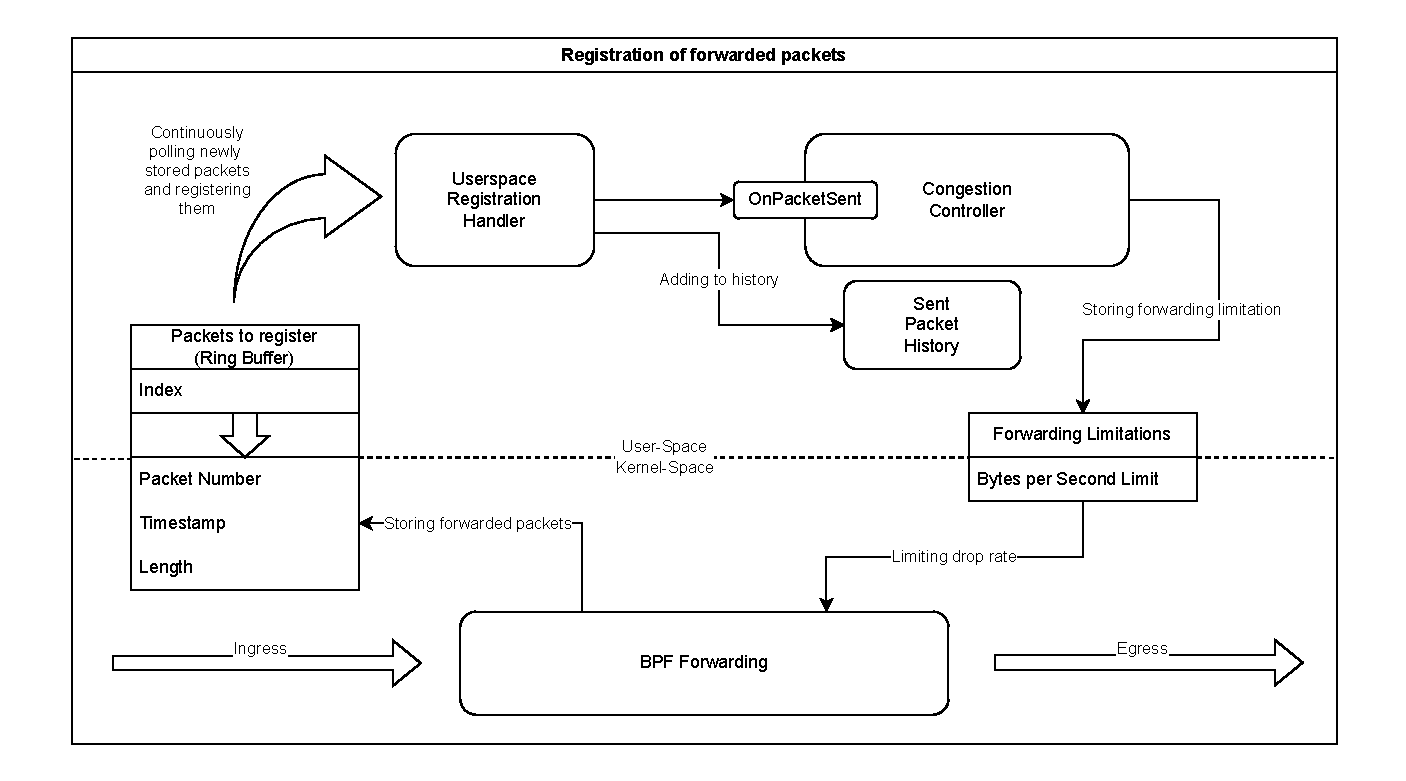
\includegraphics[width=\textwidth]{figures/03_fast_relays/forward-registration.drawio.pdf}
    \caption[Packet registration schematic]{Internal setup for registering forwarded packets as well as incorporating forwarding
    limitations for the BPF program.}\label{fig:forward-registration}
\end{figure}



TODO:~mention
\begin{figure}[htbp]
    \centering
    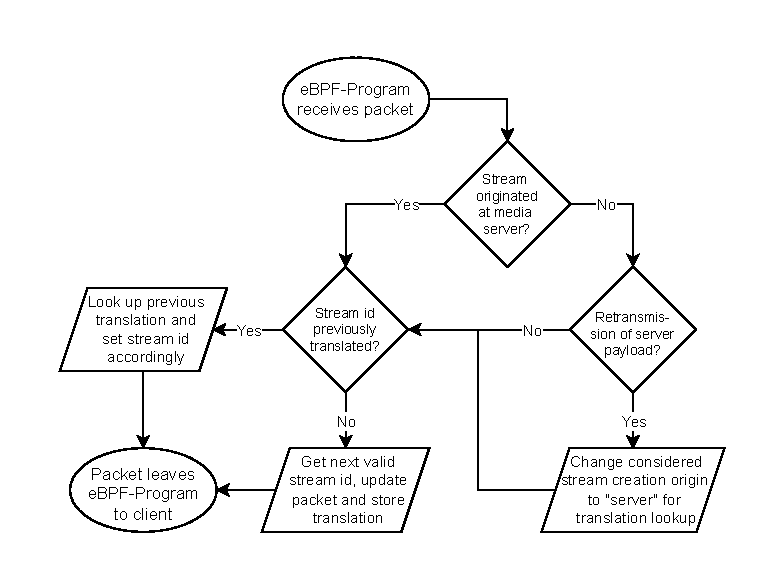
\includegraphics[width=0.8\textwidth]{figures/03_fast_relays/stream-id-translation.drawio.pdf}
    \caption[Stream id translation schematic]{TODO (also mention that the check for previous translation is needed since >1 packets per unistream are possible)}\label{fig:stream-id-translation}
\end{figure}